\documentclass[a4paper, 10pt, conference]{ieeeconf}      % Use this line for a4
\IEEEoverridecommandlockouts                              % This command is only
\overrideIEEEmargins
% \usepackage{graphics} % for pdf, bitmapped graphics files
\usepackage{graphicx}
\usepackage{subfigure}
% \usepackage{subfig}
\usepackage{float}
\title{\LARGE \bf
Measuring Social Functions of City Regions from Large-scale Taxi Behaviors
}
% \author{Lei Wang% <-this % stops a space
% }

\author{ \parbox{3 in}{\centering Lei Wang*\\
        Xi'an University of Science and Technology\\
        {\tt\small panda-wl@foxmail.com}}
}

%%%%%%%%%%% begin---doc %%%%%%%%%%%%%%%%%%%%%%%
\begin{document}
\maketitle
\thispagestyle{empty}
\pagestyle{empty}

\begin{abstract}

City-scale human mobility analysis is an important problem in pervasive computing. In this paper, with qualitative and quantitative analysis, we establish and confirm the relationship between the get-on/off characteristics of taxi passengers and the social function of city regions. We find that get-on/off amount in a region can depict the social activity dynamics in that area, i.e. the temporal variation of get-on/off amount can characterize the social function of a region. The experimental results on a large-scale real-world taxi dataset suggest that three typical regional categories can be recognized even using a very simple classification method.

\end{abstract}

%%%%%%%%%%%%%%%%%%%%%%%%%%%%%%%%%%%%%%%%%%%%%%%%%%%%%%%%%%%%%%%%%%%%%%%%%%%%%%%%
\section{INTRODUCTION}%第一章

The analysis on mass and widespread human activities draws attention of more and more researchers. Taxi trace data (GPS data) can reflect urban traffic activity and thus is widely used in traffic analysis. We observe that taxi data convey lots of information about human traces which provide the following activities:

\begin{itemize}

\item Traffic requirement: Get-on/off amount is relative to the traffic requiremen and time-variant activity pattern of a region.
\item Regions’ social function: Temporal variation of get-on/off amount in a region characterizes the social function of the region.
\item City dynamic: Get-on/off amount variation of regions describes the city’s social activity dynamics.

\end{itemize}

The correlation between taxi trace data and social activity dynamics has many promising applications: (1) It can help governments to learn city dynamics and make the city planning more reasonable. (2) It can assist taxi drivers to learn driving strategies to find passengers in an optimal way. (3) It can help passengers to find out where they should wait for a taxi, and how long they will probably take on waiting.
Motivated by these potential applications, this paper attempts to analyze get-on/off amounts using a city-scale realworld taxi GPS data set, and to establish the relationship between taxi GPS data and regions’ social functions. The contributions are in two-fold: (1) In a city-scale, we show that the get-on/off amount could depict social activity intensity of a city. (2) After qualitative analysis, we find an approach to recognize regions’ social function with temporal variation patterns of get-on/off amount. As far as we know, our work is the first time to measure social functions of regions using taxi GPS data.

Taxi traces can help better understand the urban mobility as it contains the origins and destinations of the passengers with greater accuracy compared with other public transportations e.g. bus, metro. It is a unique transportation service in a way that it is not bounded to a pre-determined path or pick-up and drop-off locations. On the other hand, it is also important to consider the reasons that people use taxis instead of other public transportations. The reasons could possibly be the lack of public transportation alternatives, the urgency of the trip, the amount of luggages, or even simple commodity.

%%%%%%%%%%%%%%%%%%%%%%%%%%%%%%%%%%%%%%%%%%%%%%%%%%%%%%%
\section{RELATED WORKS}%第二章

User trace data (e.g. GSM trace and Wi-Fi data) and traffic trace data are two main kinds of trace data used for social mobile analysis. GSM data in phones can be used for localization, thus, it can be used to analyze crowd activity and human activity pattern. Wi-Fi network activity data could be used to analyze indoor human activity, Calabrease et.al.  use MIT Wi-Fi data to cluster the buildings in MIT campus and analyze activity strength in buildings.
Taxi and shared bicycle data are important traffic trace data for social analysis. Previous research mainly tried to use the data only for traffic analysis. Many researches before developed a statistical physics approach to build a mathematical model using differential equations . Popular models include fluid-dynamical theories, kinetic theories, car-following theories, coupled-map lattice models, NagelSchreckberg cellular automata model and extensions of the NaSch model; Chowdury et.al.  gave a review of these models.
Recently, traffic data is considered in social activity studies. Ge et.al.  studied taxi drivers’ pick-up behavior using graph theory view and recommend the statistical best route for taxi drivers. Shared bicycle is also an important traffic service in some cities; people can cluster stations according to the variation of the amount of left bicycles. Such variation is also predictable by probability graphical model according to Froehlich et.al.  Kaltenbrunner  did a similar work but use an ARMA (Auto-Regressive and Moving Average) model for prediction.

%%%%%%%%%%%%%%%%%%%%%%%%%%%%%%%%%%%%%%%%%%%%%%%%%%%%%%%%%%%
\section{TAXI GPS DATASET AND PREPROCESSING}%第三章

\subsection{Dataset Description} 

Our dataset contains over than 10 million taxi-GPS samples from August to December 2009, collected in Lisbon by GeoTaxi. The data sampling rate varies according to the trip nature. Samples can be stored according to the distance covered by the vehicle, time elapsed or when some state changed (e.g. occupancy). For the study purposes, only the pick-up and drop-off location and timestamp are considered, corresponding to 271,172 distinct trips. The data was collected from 253 distinct taxis, which account for nearly 15\% of taxis in Lisbon area. 

The area of study encompasses the Lisbon council, consisting of 53 parishes, an area around 110 km2, with a population of 800,000. The urban area growth in several layers around the city downtown, the central point, which includes the oldest and smallest parishes with greatest population density, touristic, historic and commercial areas, and the interface for several public transportation services (bus, metro, train and ferry).  In the marginal avenue around Tagus River, there are touristic, recreational and commercial areas. Moving away from the city center we find greater parishes with lower population density, characterized by residential areas around business areas. Major infrastructures (e.g. airport, industrial facilities) are located in the city’s periphery. For the analysis, we model the Lisbon map with grids of 0.5x0.5 km2. 

The overall taxi service distribution in Lisbon can be seen in Fig.\ref{fig:my_png_1} where some major locations such as the city downtown (A), the airport (B), and the train station (C) are identified.  

\begin{figure}[ht]
    \centering
    \subfigure[Pick-up locations]{
        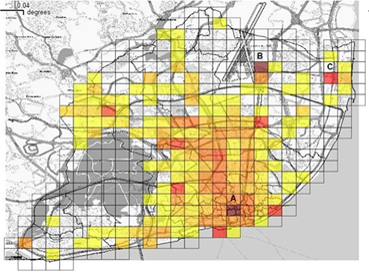
\includegraphics[width=0.22\textwidth]{fig/png1_a.png}
    } 
    % \vspace{0.01cm}
    \subfigure[Drop-off locations]{
        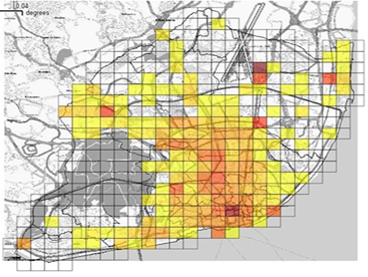
\includegraphics[width=0.22\textwidth]{fig/png1_b.png}
    }
    \caption{ Taxi pick-up (a) and drop-off locations (b) distribution. }
    \label{fig:my_png_1}
\end{figure}

The following figure shows the temporal variation of the taxi services. As expected, it gradually increases in the morning reaches the maximum between 11 a.m. and 1 p.m, and slowly drops down in the afternoon. In the working days, there are more taxi services than in the weekends with the maximum number of the services observed on Monday. 

\begin{figure}[ht]
    \centering
    \subfigure[Hourly variation]{
        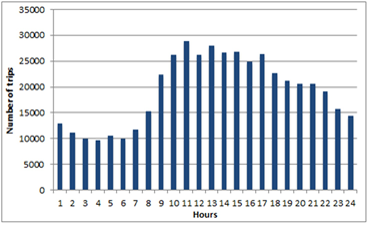
\includegraphics[width=0.22\textwidth]{fig/png2_a.png}
    } 
    % \vspace{0.01cm}
    \subfigure[Daily variation]{
        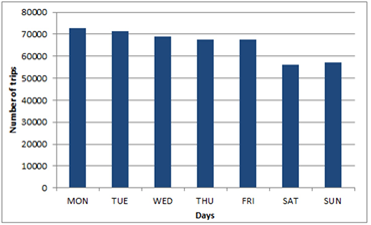
\includegraphics[width=0.22\textwidth]{fig/png2_b.png}
    }
    \caption{ Taxi service variation according to the hours of day (a) and days of week (b). Taxi service variation according to the hours of day (a) and days of week (b).}
    \label{fig:my_png_2}
\end{figure}

The taxi dataset used in this paper comes from the Hangzhou City Traffic Bureau, which were generated by GPS devices on taxis during the period of nearly a year (from April 1st, 2009 to April 20th, 2010). At this period, the number of taxis installed GPS device increases from 4597 to 7475, while the total number of taxis in the city keeps almost unchanged. The dataset has about 3 billion records; most of them were sampled at a frequency of about 1 minute. Each record consists of the following information:

\begin{itemize}

\item TAXI ID: the unique ID of each taxi;
\item TIME: the sampling time, with the timestamp format of ’YYYY-MM-DD HH:MM:SS’;
\item GPS POSITION: the longitude and the latitude at the sampling time;
\item SPEED: the taxi speed in km/h at the sampling moment; • TAXI ORIENTATION: the direction the taxi facing to, from 0 to 360 in clockwise with zero for the north;
\item GPS STATE: it sets to one when GPS data is wrong, and sets to zero otherwise. In our experiment, all the records with wrong GPS data are filtered.
\item METER STATE: indicates whether the taximeter is running, i.e. whether there is a passenger on the taxi or not.

\end{itemize}

\subsection{Data Cleaning and Preprocessing}
Here we describe our data cleaning process. Based on our original dataset, a distribution of the trip distances is shown in Fig.\ref{fig:my_png_3}. We notice that that the realistic longest trips could be around 22km (one side of the city to the other), we thus discarded trips with distance greater than 30km. On the other hand, the original data also contains a great amount of trips with less than 200m (14.94\% of the all trips), which seems unrealistic. Therefore, in addition, we discarded these small trips from our analysis.  
\begin{figure}[ht]
    \centering
    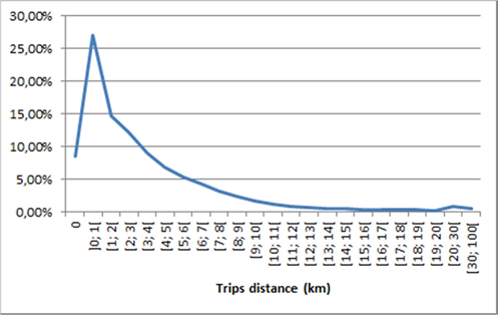
\includegraphics[width=7cm]{fig/png3.png}
    \caption{ Distribution of trips distances. }
    \label{fig:my_png_3}
\end{figure}
The trip duration distribution is represented by the following figure. Similar to the trip distance distribution, we discarded trips that are less than one minute and longer than two hours. After the data cleaning process, we retained 177,169 trips and 217 distinct taxis. 
 \begin{figure}[ht]
    \centering
    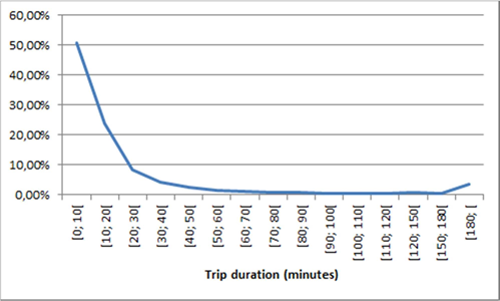
\includegraphics[width=7cm]{fig/png4.png}
    \caption{Distribution of trips duration. }
    \label{fig:my_png_4}
\end{figure}


Get-on/off amount information is important in taxi traces data because it can depict human mobility characteristics in a region. This subsection shows how we get get-on/off amount of a defined region from mass of taxi traces. • Sampling: We randomly sample 4000 taxis for analysis since the number of taxis that install GPS device does not keep constant in the observed year.

\begin{itemize}

\item City Map Partition: This paper chooses the map area of [30.15, 30.40] for the north latitude and [119.9, 120.4] for the east longitude, since the Hangzhou city mainly locates within this area. We divide the chosen area into 250×500 regions with 100×100 square for each region. The region size of 100 meters is determined because larger areas may have multiple social functions while smaller areas may be nonsense considering that the precision of GPS data is usually tens of meters.
\item Get-On/Off Counting: Transition of the meter state reflects that passengers are getting on or off. We eliminate state transition noises by setting a time threshold for state transition from 0 to 1. Then we extract the get-on/off amount from data, by simply counting the number of transitions occurred in a defined area.

\end{itemize}

%%%%%%%%%%%%%%%%%%%%%%%%%%%%%%%%%%%%%%%%%%%%%%%%%%%%%
\section{USING THE TEMPLATE}%第四章

Get-on/off amounts’ temporal variation contains rich information regarding to urban and regional social dynamics. We find that daily get-on/off amount in the city varies according to citizens’ daily social activity intensity. Total amount of geton/offs in different days can highlight important social activity in some uncommon days. Moreover, regions with different social function show very different pattern of get-on/offs.

\subsection{City-wide Dynamics Analysis} For the city-wide statistics, the total get-on/off amount variation over days can reflect social meaning of some uncommon days such as holiday and school-open days.
The total get-on/off amount in different days can highlight uncommon days that have important social activities (Fig. \ref{fig:my_label_1}). At the peak in August 2009, schools open and students come back to or freshman enters the school. During the Spring Festival, people may stay at home and seldom travel around by taxi. And, the decrease in the National Day is caused by traffic jam, since too many people may go outside during that day.

\begin{figure}[ht]
    \centering
    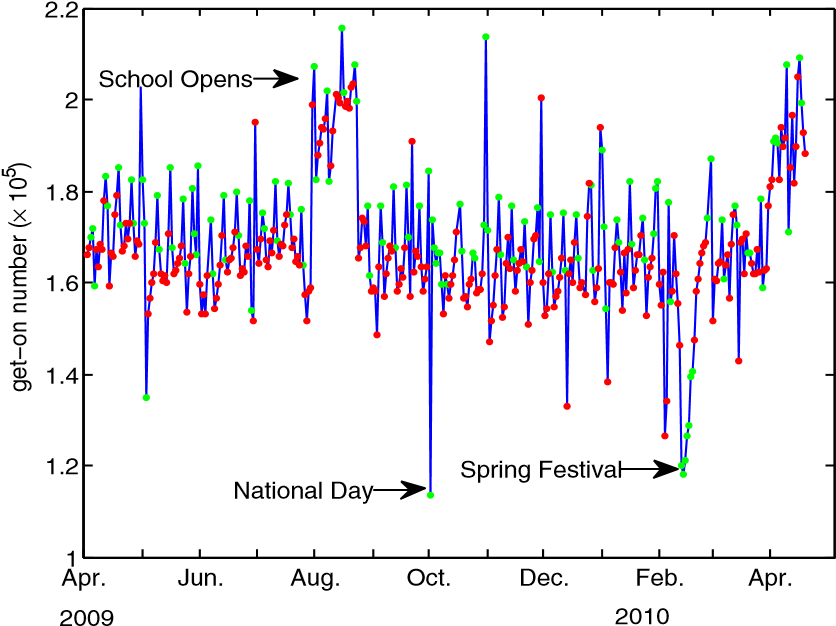
\includegraphics{fig/f1.png}
    \caption{Illustration of city-wide dynamics: total get-on/off amount variation over different days.}
    \label{fig:my_label_1}
\end{figure}

\subsection{Regional Social Functions Analysis}Besides the city-wide analysis, statistics of region-wide in a city may also exhibit patterns of human activity in the area. By qualitatively analyzing get-on/off amount in several time periods in a day, we observe that regions with different social function have their distinctive temporal variation patterns.
This paper preliminary considers three typical categories of regions: (1) coach/train stations; (2) entertainment districts; (3) scenic spots. Fig. \ref{fig:my_label_2} illustrates:

\begin{itemize}

\item Train stations: Train stations are very hot in almost all the time over the whole day.
\item Scenic spots: Tourists often go to scenic spots only during the daytime.
\item Entertainment districts: People usually go for entertainment mainly at night; few people will go there at dawn and seldom any passengers travel there in the morning.

\end{itemize}

The analysis above confirms relationship between regional taxi get-on/off amount and social activity in a region. The features of three types of regions we got by qualitative analysis conform to common sense. They show that taxi passengers are a kind of representative samples from citizens, and taxi get-on/off amount depicts human activity strength in a region. Besides, these examples show very different features of geton/off amount temporal variation for different types of regions, and hence the feasibility of recognizing social function of regions using temporal variation of get-on/off amount.

\subsection{Trip distance distribution}After the data cleaning process, we examine the trip distance distribution (Fig.\ref{fig:my_png_5}) and find that we can fit it with a Gamma distribution with $ \alpha =2.7 $ and $\beta =1.2 $ as following:
 \begin{equation}
 	f_{\alpha,\beta}(x)=\frac{1}{\Gamma(\alpha)\beta^{\alpha}}x^{\alpha-1}e^{\frac{\alpha}{\beta}}
    \label{eq:quadratic}
\end{equation}

\begin{figure}[ht]
    \centering
    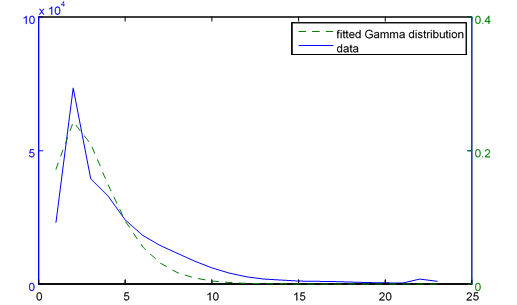
\includegraphics{fig/png5.png}
    \caption{Distribution of trips distance (solid line) and fitted Gamma distribution (dashed line). }
    \label{fig:my_png_5}
\end{figure}

If the first interval is removed, we can represent it with an exponential distribution, exp(λ) with λ = 0.26 (Fig. 6). The same phenomenon (exponential distribution) can also be observed for the trip duration and the trip income. 

\begin{figure}[ht]
    \centering
    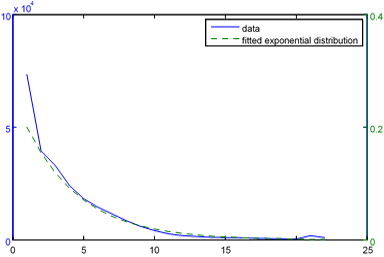
\includegraphics{fig/png6.png}
    \caption{Trip distance distribution without the first interval of the dataset (solid line) and fitted exponential distribution with λ = 0.26 (dashed line).}
    \label{fig:my_png_6}
\end{figure}

\subsection{Driver strategies} We find that the majority of the taxi drivers appear to be using combined strategies – mainly driving around the city and in certain time periods staying at a fixed location. This phenomenon can be observed in the Fig. \ref{fig:my_png_7} where there is an increase of trips from the airport between 6 a.m. and 8 a.m. and elsewhere in other time slots. On the other hand, in the same period there is a significant decrease of trips from the remaining locations.  


To confirm our observation, we examine mobile phone data collected from GSM networks. The GSM data consists of samples from November and December 2009 providing statistical measures of carried load (Erlang) with one-hour period. In Fig. \ref{fig:my_png_8}, we can observe that immediately after the taxi rush hour there is an increase of the GSM network usage in the airport, while the mobile phone activities in other locations of the city begins to arise three hours later. This is an indication of the possible taxi passengers at airport. 

\begin{figure}[ht]
    \centering
    \subfigure[Hourly variation]{
        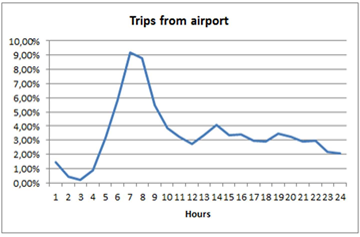
\includegraphics[width=0.21\textwidth]{fig/png7_a.png}
    } 
    % \vspace{0.01cm}
    \subfigure[Daily variation]{
        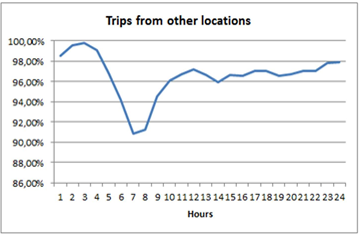
\includegraphics[width=0.21\textwidth]{fig/png7_b.png}
    }
    \caption{ TVariation of number of trips aggregated by hour. Left:  pick-up location from the airport. Right: pick-up from other locations. }
    \label{fig:my_png_7}
\end{figure}

\begin{figure}[ht]
    \centering
    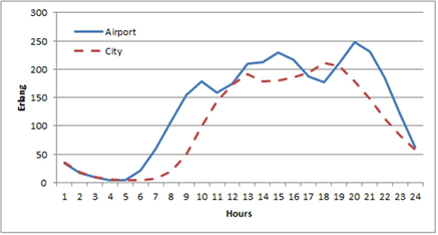
\includegraphics{fig/png8.png}
    \caption{GSM network usage aggregated by hour. }
    \label{fig:my_png_8}
\end{figure}

%%%%%%%%%%%%%%%%%%%%%%%%%%%%%%%%%%%%%
\section{SOCIAL FUNCTION RECOGNITION FOR REGIONS}%第五章
Section IV confirms qualitatively the relationship between regional get-on/off amount and human activity intensity. In this section, we analyze quantitatively the relationship between get-on/off amount and regions’ social function. With a simple classification method, we recognize precisely regions’ social function and find corresponding get-on/off amount time domain patterns.
\begin{figure}[ht]
    \centering
    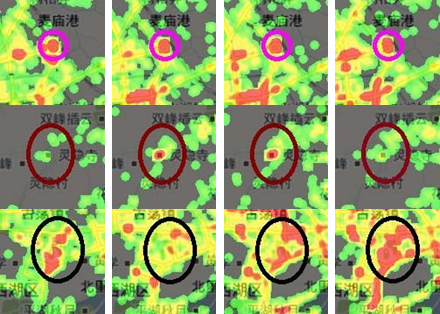
\includegraphics{fig/f2.png}
    \caption{Illustration of variation of passengers get-off number over time for three region categories. The grayscale of color represents density of get-on/off number. Each row is for one region category: train station, scenic spot and entertainment districts (from top to bottom).}
    \label{fig:my_label_2}
\end{figure}
\subsection{Data Labeling} For data preparation, we find three taxi drivers to label typical regions of each category with pure social function. We finally get 76 regions with pure social function in total and use them for further analysis. The labeled regions include 37 regions near train/coach station, 27 entertainment districts, and 12 scenic spots.

\subsection{NTF: Mobility patterns}Since our data tensor has three dimensions, the decomposition returned three different components which determine the scale of mobility flow in each dimension for every cluster: time (hour of week) and space (departure and arrival tracts). Thus, individual clusters represent groups of taxi rides in different places at different periods of time in a weekday-hour scale.

The time component is shown in Figure 1a, whereas location components for pickups (departures) and drop-offs (arrivals) are shown on the right-hand side of Fig. \ref{fig:my_png_9}. Due to space limitations we show only the first three clusters. From Fig. \ref{fig:my_png_9}, it can be observed that all clusters show strong daily regularities, which can be assumed as daily routines in human mobility behavior. Clusters C1,C2,C4,C5 andC7 capture all behaviors on workdays (almost all peaks are within the first five days of the week), whereas clusterC3 is strongly dominated by weekends, specially by Friday and Saturday nights. Cluster C6 on the other hand, shows a more periodical behavior across the entire week, however its peaks are around 6pm from Monday to Saturday and 2pm on Saturdays and Sundays.

\begin{figure}[ht]
    \centering
    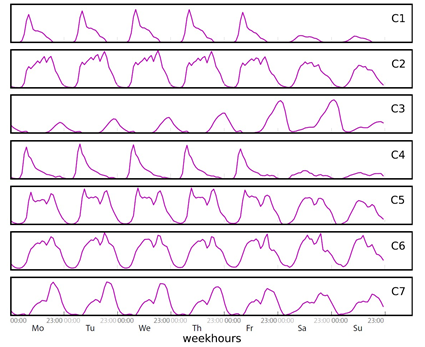
\includegraphics{fig/png9.png}
    \caption{Temporal distribution of clusters}
    \label{fig:my_png_9}
\end{figure}

\subsection{Recognition of Social Function}Two types of features are considered: coarse-grained feature and fine-grained feature. Given n days data, the coarse-grained feature is a n-dimension vector with daily total amount of geton/off as element. The fine-grained feature is a 4n-dimension vector with four get-on/off numbers for four time periods in each day: (a) 6:30 a.m. to 8:30 a.m.; (b) 9:00 a.m. to 3:00 p.m.; (c) 7:00 p.m. to 9:00 p.m.; (d) 11:00 p.m. to 1:00 a.m. These four time periods are extracted according to the largest variance of amount. The recognition process is as follows:

\begin{itemize}

\item Feature Vector: The feature vectors are defined as $ x^{i}_{d} $ and $ x^{i}_{u} $ which represent the amount of get-on or get-off in the $i$th region $D_i$ with elements $ x^{i}_{u}(j) $ and $ x^{i}_{d}(j) (j=1,2,...) $.
\item Normalization: Normalization is to centralize the feature vector $ x^{i}_{u}(j)=x^{i}_{u}(j)-\Sigma_{j}x^{i}_{u}(j)/n $, and $ x^{i}_{d}(j)=x^{i}_{d}(j)-\Sigma_{j}x^{i}_{d}(j)/n $.
\item Similarity definition: We define similarity $ s_{i,j} $ between each two regions $ D_i $ and $ D_j $: $ s_{i,j}=max(cos(x^{i}_{u},x^{j}_{u}),cos(x^{i}_{d},x^{j}_{d})) $, where $ cos(x^i,x^j) $ is the cosine similarity of the two normalized vectors: $ x^i $ and $ x^j $.
\item Agglomerative clustering: Agglomerate samples with enough large similarity (similarity threshold) into the same cluster. Some samples may be not much similar (similarity below the threshold) to the clusters and thus belong to none of the clusters. These samples are classified according to the most similar sample in clusters.
\item Recognition: Test samples are clustered together with training samples as above. Label the test sample according to voting by the number of training sample in the same cluster.

\end{itemize}

\subsection{Experimental Result and Analysis}

\subsubsection{Feature vector visualization}The coarse-grained feature vector extracted from one year data is visualized in Fig. \ref{fig:my_label_3}

\begin{itemize}
\item Scenic spots. They show very different pattern between holidays and weekdays, they have much more passengers in holiday than weekdays (Fig. \ref{fig:my_label_3}a).
\item Train/coach station. Get-on/off amount of stations highlights some uncommon time points instead of difference between workdays and weekdays (Fig. \ref{fig:my_label_3}b).
\item Entertainment districts. They are similar to scenic spots but the variance between the peaks and the troughs is small (Fig. \ref{fig:my_label_3}c).

\end{itemize}

\begin{figure}
    \centering
    \subfigure[]{
        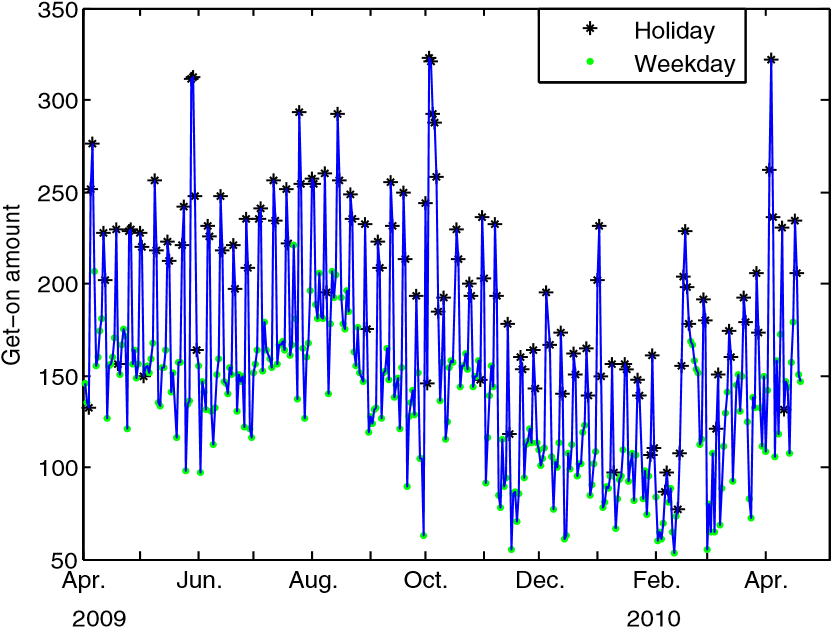
\includegraphics{fig/f3.png}
    }
    \subfigure[]{
        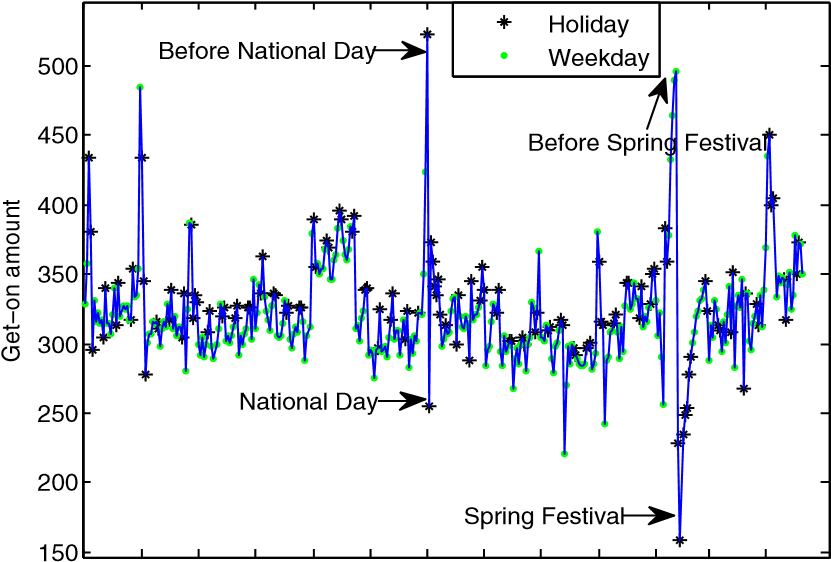
\includegraphics{fig/f4.png}
    }
    \subfigure[]{
        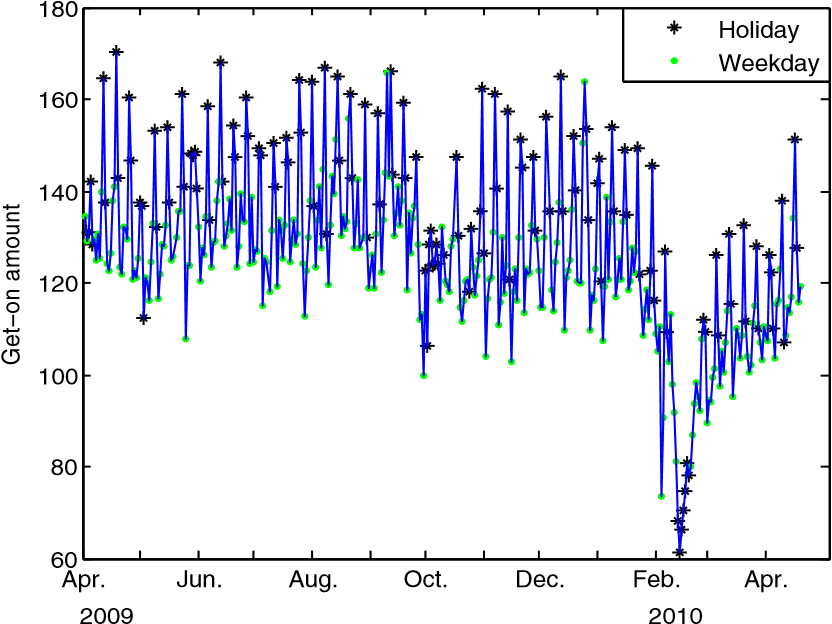
\includegraphics{fig/f5.png}
    }
    \caption{Visualization of feature vectors for the three region categories (a) scenic spots, (b) stations and (c) entertainment districts. All the get-on number is averaged over the regions of the same category.}
    \label{fig:my_label_3}
\end{figure}

We also reduce the dimension of feature vectors by the principal component analysis and visualize the regions in the 3D-Eigenspace. In Fig. \ref{fig:my_label_4}, samples with different region categories scatter apart from each other.

\begin{figure}[htbp]
    \centering
    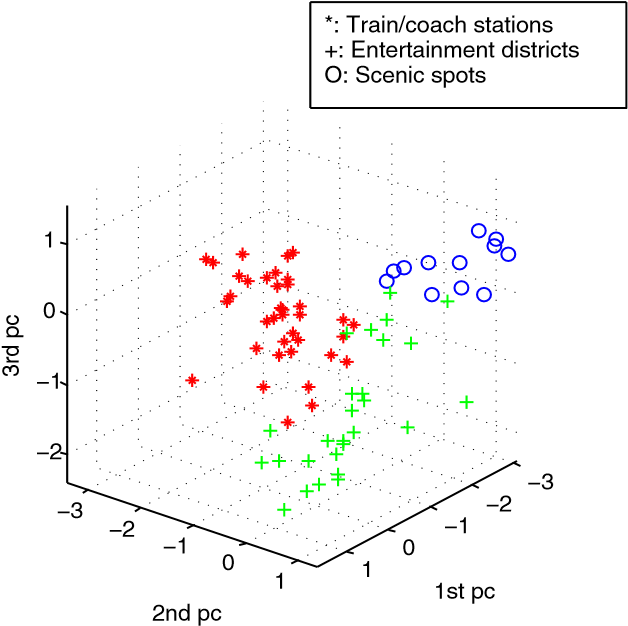
\includegraphics{fig/f6.png}
    \caption{Illustration of the labeled samples of three typical region categories in the 3D Eigenspace.}
    \label{fig:my_label_4}
\end{figure}
\begin{figure}[ht]
    \centering
    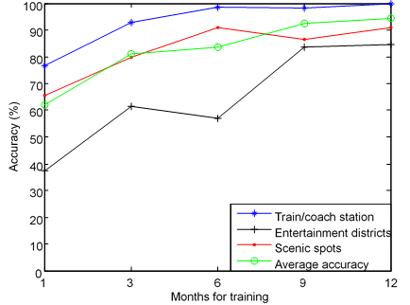
\includegraphics{fig/f7.png}
    \caption{Recognition performance of coarse-grained feature with varying data amount for training.}
    \label{fig:my_label_5}
\end{figure}

\subsubsection{ Recognition result and analysis}The recognition result is listed in Table I. Our method can recognize social function of the regions precisely. Moreover, there are some interesting conclusions we can get from this result: The tow types of features can be recognized more precisely with more data added. The recognition accuracy using coarse-grained feature grows quickly 5, while the accuracy using fine-grained feature changes slowly.

\begin{itemize}
\item For short time-span data (one week and one month), fine grained feature vector can be recognized more precisely since it considers different time periods during a day. For long time-span data (one year), coarse-grained feature vector has higher recognition accuracy.
\item The coarse-grained feature vector extracted from one year data can be best recognized. The average recognition accuracy using this feature is 94.44\%.

\end{itemize}

\begin{table*}[h] %开始一个表格environment,表格的位置是h,here。
\centering
\caption{RECOGNITION ACCURACY BY VARYING FEATURE TYPES AND TRAINING DATA AMOUNT} %显示表格的标题
\begin{tabular}{c|c|c|c|c|c}
	\hline 
	& Data for & Train/Coach & Entertainment & Scenic & Average \\ 
	\hline 
	Feature Types &  &  &  &  &  \\ 
	& Training & Station & Districts & Spots & Accuracy \\ 

	\hline 
	 & one week & 53.85\% & 37.79\% & 26.02\% & 44.00\% \\ 

	Coarse-grained feature & one month & 76.65\% & 37.40\% & 65.42\% & 61.94\% \\ 
 
	& one year & 100.00\% & 84.62\% & 90.91\% & 94.44\% \\ 
	\hline 
	& one week & 82.37\% & 89.43\% & 72.50\% & 83.32\% \\ 

	Fine-grained feature & one month & 84.49\% & 86.56\% & 68.53\% & 82.68\% \\ 

	& one year & 88.89\% & 92.31\% & 81.82\% & 89.04\% \\ 
	\hline 

\end{tabular} 
\end{table*}

The results show that regions’ social function can be recognized correctly and these regions have clear temporal patterns. To sum up, by recognition, we reveal that, from a quantitative view, social function and regional get-on/off amount are indeed tightly related.

\section{DISCUSSION}
In this work, we have shown that spatio-temporal dynamics in human behavior can potentially be better explained by considering parts of the data separately. We identified clusters of taxi rides and utilized openly available data from the Web to explain them. However, there are some aspects that need to be taken into account for the current approach.

\begin{itemize}

\item Concentration parameter k. As discussed in [33], the HypTrails approach requires setting a parameter k to elicit Dirichlet priors from hypotheses. Higher values of k express stronger believes in the respective hypotheses. Technically, larger values of k imply higher values of the hyperparameters (pseudo counts) of the Dirichlet distributions. In our experiments, we tried several values of k from 0 to 100; overall very similar results. The reported results in this paper use an intermediate value of k = 10.
\item Correlations in the explanations. Using HypTrails to explain clusters will not be able to identify causes of movement patterns, but only correlations. As an example, for Cluster C2 in our case study the Art Galleries hypothesis performs best. This of course does not mean that taxi trips in that cluster prominently have art galleries as destinations, but that people go to places that also have nearby art galleries. In that direction, we also intend to integrate a correlation analysis between the used hypotheses in future work in order to identify explanations that are similar to each other.
\item Clustering method. In this paper, we use HypTrails to explain clusters obtained by Non-negative tensor factorization. While NTF is a reliable and established method in this line of research, the clustering approach is exchangeable and could be replaced by any other clustering technique.
\item State space. Since our approach requires a discrete state space, it is necessary to aggregate pick-up and drop-off locations of the taxi rides in an area. The choice of these aggregational units (i.e., the states in our state space) can potentially influence the results. This is known in literature as the Modifiable areal unit problem. In this paper, we chose tracts for the level of our analysis as it allowed for the direct integration of information from census data. Experiments with different state spaces are subjects of future work.
\item Multiple dimensions. In this paper, we cluster taxi trips with respect to time, pick-up and drop-off location. However, our approach allows to extend these by additional information, e.g., number of passengers. In this case, a higher dimensional tensor would be used by NTF, but the resulting clusters could also be explained with help of the HypTrails approach. The scale of these dimensions could also suggest more fine-grained mobility behaviors. For instance, in this work we defined the time dimension as all 168 hours of a week in order to distinguish patterns on workdays and weekends.
\item Normalization. The external online data we use for constructing mobility hypotheses might not be evenly distributed across all tracts. Therefore the HypTrails approach normalizes each belief matrix to be able to compare different hypotheses to each other.
\end{itemize}

\section{CONCLUSION AND FUTURE WORK}%第六章
This paper investigates the relationship between regional get-on/off amount and regions’ social function. Firstly, from a city scale, the get-on/off amount variation in a day or among different days conforms to social activity intensity of citizens. Secondly, from a qualitative view, regional get-on/off amount daily variations are very different in regions with different social functions.
Based on the investigation, we develop a simple method to recognize regions’ social function. The preliminary results on a large-scale real-world taxi GPS data set show that our approach achieves recognition accuracy of 94.44%.
There is still much further work to do in the work-inprogress. Firstly, our regions are rigid squares which may not represent a intact region in the city. Thus, we are going to develop new methods to get more natural regions. Secondly, we consider only three types of regions. More social function classes should be added and more regions should also be considered. Finally, we consider regions with pure social function in this paper while regions are more complicate in reality.

Analyzing the taxi traces from Lisbon, Portugal during a period of five months, we are able to capture the spatiotemporal variation and observe that trip distance, duration, and income follow Gamma and Exponential distribution. We also examine taxi driving strategies where a combination of pick-up customers around the city and in fixed locations is observed. There are clearly rooms for improvements and further investigations for this preliminary study. As our future work, we will continue to investigate on how taxi traces can be useful for urban planning and transportation management. We will also explore into data visualization and multi-source data fusion – integrating taxi data with other public transportation such as bus, metro, and fleets as well as mobile phone data to better understand the mobility and flow of the city. 

\addtolength{\textheight}{-12cm}   % This command serves to balance the column lengths
                                  % on the last page of the document manually. It shortens
                                  % the textheight of the last page by a suitable amount.
                                  % This command does not take effect until the next page
                                  % so it should come on the page before the last. Make
                                  % sure that you do not shorten the textheight too much.

%%%%%%%%%%%%%%%%%%%%%%%%%%%%%%%%%%%%%%%%%%%%%%%%%%%%%%%%%%%%%%%%%%%%%%%%%%%%%%%%
\begin{thebibliography}{99}

\bibitem{} M. Becker, P. Singer, F. Lemmerich, A. Hotho, D. Helic, and M. Strohmaier. Photowalking the city: Comparing hypotheses about urban photo trails on Flickr. In Int. Conference on Social Informatics, 2015.
\bibitem{} C. Brettell and J. Hollifield. Migration Theory: Talking Across Disciplines. Taylor \& Francis, 2014.
\bibitem{} G. Chen, X. Jin, and J. Yang. Study on spatial and temporal mobility pattern of urban taxi services. In Int. Conference On Intelligent Systems and Knowledge Engineering, 2010.
\bibitem{} A. Chua, E. Marcheggiani, L. Servillo, and A. V. Moere. FlowSampler: Visual Analysis of Urban Flows in Geolocated Social Media Data. In Int. Conference on Social Informatics. Springer, 2014.
\bibitem{} L. Ding, H. Fan, and L. Meng. Understanding Taxi Driving Behaviors from Movement Data. In AGILE 2015, pages 219–234. Springer, 2015.
\bibitem{}B. Donovan and D. B. Work. Using coarse gps data to quantify city-scale transportation system resilience to extreme events. arXiv:1507.06011, 2015.
\bibitem{}D. Falcone, C. Mascolo, C. Comito, D. Talia, and J. Crowcroft. What is this place? Inferring place categories through user patterns identification in geo-tagged tweets. In Int. Conference on Mobile Computing, Applications and Services, 2014.
\bibitem{}N. Ferreira, J. Poco, H. T. Vo, J. Freire, and C. T. Silva. Visual exploration of big spatio-temporal urban data: A study of new york city taxi trips. Transactions On Visualization and Computer Graphics, 19(12):2149–2158, 2013.
\bibitem{}L. Gabrielli, S. Rinzivillo, F. Ronzano, and D. Villatoro. From tweets to semantic trajectories: mining anomalous urban mobility patterns. In Citizen in Sensor Networks, pages 26–35. Springer, 2014.
\bibitem{}L. Gauvin, A. Panisson, A. Barrat, and C. Cattuto. Revealing latent factors of temporal networks for mesoscale intervention in epidemic spread.
\bibitem{}L. Gauvin, A. Panisson, and C. Cattuto. Detecting the community structure and activity patterns of temporal networks: a non-negative tensor factorization approach. PloS One, 9(1), 2014.
\bibitem{}N. Hao, L. Horesh, and M. Kilmer. Nonnegative Tensor Decomposition. In Compressed Sensing \& Sparse Filtering, pages 123–148. Springer, 2014.
\bibitem{}C. K. Vaca, D. Quercia, F. Bonchi, and P. Fraternali. Taxonomy-Based Discovery and Annotation of Functional Areas in the City. In Int. Conference on Web and Social Media, 2015.
\bibitem{}J. L. Toole, M. Ulm, M. C. González, and D. Bauer. Inferring land use from mobile phone activity. In Int. Workshop on Urban Computing, 2012.
\bibitem{}K. Takeuchi, R. Tomioka, K. Ishiguro, A. Kimura, and H. Sawada. Non-negative multiple tensor factorization. In Int. Conference on Data Mining, 2013.
\bibitem{}C. Song, Z. Qu, N. Blumm, and A.-L. Barabási. Limits of predictability in human mobility. Science, 327(5968):1018–1021, 2010.
\bibitem{}P. Singer, D. Helic, A. Hotho, and M. Strohmaier. HypTrails: A Bayesian Approach for Comparing Hypotheses About Human Trails on the Web. In Int. Conference on World Wide Web, 2015.
\bibitem{}F. Simini, M. C. González, A. Maritan, and A.-L. Barabási. A universal model for mobility and migration patterns. Nature, 484(7392):96–100, 2012.
\bibitem{}A. Sarkar, N. Lathia, and C. Mascolo. Comparing citiesâA˘ Z cycling patterns´ using online shared bicycle maps. Transportation, 42(4):1–19, 2015.
\bibitem{}V. Salnikov, R. Lambiotte, A. Noulas, and C. Mascolo. OpenStreetCab: Exploiting Taxi Mobility Patterns in New York City to Reduce Commuter Costs. arXiv:1503.03021, 2015.
\bibitem{}A. Noulas, B. Shaw, R. Lambiotte, and C. Mascolo. Topological Properties and Temporal Dynamics of Place Networks in Urban Environments. In Int. Conference on World Wide Web Companion, 2015.
\bibitem{}A. Noulas, S. Scellato, C. Mascolo, and M. Pontil. An Empirical Study of Geographic User Activity Patterns in Foursquare. 2011.
\bibitem{}A. Noulas, S. Scellato, R. Lambiotte, M. Pontil, and C. Mascolo. A tale of many cities: universal patterns in human urban mobility. PloS One, 7(5):e37027, 2012.
\bibitem{}X. Liu, L. Gong, Y. Gong, and Y. Liu. Revealing daily travel patterns and city structure with taxi trip data. arXiv:1310.6592, 2013.
\bibitem{}X. Li, G. Pan, Z. Wu, G. Qi, S. Li, D. Zhang, W. Zhang, and Z. Wang. Prediction of urban human mobility using large-scale taxi traces and its applications. Frontiers of Computer Science, 6(1):111–121, 2012.
\bibitem{}Lenormand, Maxime and Gonçalves, Bruno and Tugores, Antònia and Ramasco, José J. Human diffusion and city influence. arXiv:1501.07788, 2015.
\bibitem{}R. Jurdak, K. Zhao, J. Liu, M. AbouJaoude, M. Cameron, and D. Newth. Understanding Human Mobility from Twitter. arXiv:1412.2154, 2014.
\bibitem{}S. Jiang, J. Ferreira, and M. C. González. Clustering daily patterns of human activities in the city. Data Mining and Knowledge Discovery, 25(3):478–510, 2012.
\bibitem{}L. Wu, Y. Zhi, Z. Sui, and Y. Liu. Intra-urban human mobility and activity transition: evidence from social media check-in data. PloS One, 9(5), 2014.
\bibitem{}K. Willis. Introduction: mobility, migration and development. Int. Development Planning Review, 32(3-4):i–xiv, 2010.
\bibitem{}Yuan, J., Zheng, Y., Zhang, C., Xie, W., Xie, X., Huang, Y.:T-Drive: Driving Directions Based on Taxi Trajectories, in ACM SIGSPATIAL GIS 2010, Association for Computing Machinery, Inc., 1 (2010) 
\bibitem{}Liu, L., Andris, C., Bidderman, A., Ratti, C.: Revealing taxi drivers mobility intelligence through his trace. Movement-Aware Applications for Sustainable Mobility: Technologies and Approaches pp. 105-120 (2010) 
\bibitem{}C. Peng, X. Jin, K.-C. Wong, M. Shi, and P. Liò. Collective human mobility pattern from taxi trips in urban area. PloS One, 7(4):e34487, 2012.
\bibitem{}F. Le Néchet. Urban spatial structure, daily mobility and energy consumption: a study of 34 european cities. Cybergeo: European Journal of Geography, 2012.

\end{thebibliography}

\end{document}